\documentclass[11pt,a4paper]{article}

\usepackage[margin=1in]{geometry}
\usepackage{amsmath,amssymb}
\usepackage{booktabs}
\usepackage{graphicx}
\usepackage{array}
\usepackage{longtable}
\usepackage{float}
\usepackage[hidelinks]{hyperref}

\graphicspath{{figures/}{../figures/}}

\title{Homework 1 -- Network Dynamics and Learning}
\author{}
\date{}

\begin{document}
\maketitle

\section{Introduction}

This report summarizes the computational solution of Homework 1. The first
exercise studies max-flow/min-cut structure and capacity augmentation in a
small directed network. The second exercise reconstructs an undirected graph
from the assignment figure and compares Katz centrality with a distributed
PageRank iteration. The third exercise uses the provided traffic-network data
to compute shortest paths, maximum flow, socially optimal routing, Wardrop
equilibria, and tolls that decentralize selected optima.

All numerical values reported below are taken from the generated CSV files and
the project results log. The scripts that produce these values are
\texttt{src/exercise1.py}, \texttt{src/exercise2.py}, and
\texttt{src/exercise3.py}.

\section{Exercise 1 -- Max-flow and cuts}

The network is the directed graph \(G=(V,E)\) with node set
\[
V=\{o,a,b,c,d\},
\]
source \(o\), sink \(d\), and directed capacitated edges
\[
\begin{array}{c|c|c}
\text{edge} & \text{arc} & \text{capacity}\\
\hline
e_1 & o\to a & 3\\
e_2 & a\to d & 3\\
e_3 & o\to b & 3\\
e_4 & b\to c & 3\\
e_5 & c\to d & 2\\
e_6 & a\to b & 1
\end{array}
\]

For an \(o\)-\(d\) cut \(S\subset V\), \(o\in S\), \(d\notin S\), the cut
capacity is the sum of the capacities of all directed edges leaving \(S\),
that is, edges with tail in \(S\) and head in \(V\setminus S\). Since the
intermediate nodes are \(a,b,c\), there are \(2^3=8\) possible cuts.

\begin{table}[h]
\centering
\begin{tabular}{c|c|c|c}
\hline
\(S\) & \(V\setminus S\) & Crossing edges & Capacity\\
\hline
\(\{o\}\) & \(\{a,b,c,d\}\) & \(e_1,e_3\) & 6\\
\(\{o,a\}\) & \(\{b,c,d\}\) & \(e_2,e_3,e_6\) & 7\\
\(\{o,b\}\) & \(\{a,c,d\}\) & \(e_1,e_4\) & 6\\
\(\{o,c\}\) & \(\{a,b,d\}\) & \(e_1,e_3,e_5\) & 8\\
\(\{o,a,b\}\) & \(\{c,d\}\) & \(e_2,e_4\) & 6\\
\(\{o,a,c\}\) & \(\{b,d\}\) & \(e_2,e_3,e_5,e_6\) & 9\\
\(\{o,b,c\}\) & \(\{a,d\}\) & \(e_1,e_5\) & 5\\
\(\{o,a,b,c\}\) & \(\{d\}\) & \(e_2,e_5\) & 5\\
\hline
\end{tabular}
\caption{All \(o\)-\(d\) cuts for Exercise 1(a).}
\label{tab:exercise1-cuts}
\end{table}

The minimum cut capacity is \(5\). The maximum flow value computed on the same
network is also \(5\), so the max-flow/min-cut theorem is verified for this
instance.

\subsection*{Capacity augmentation on existing links}

In part 1(b), an integer budget \(x\geq 0\) of additional capacity is
distributed among the six existing links. For each \(x=0,\ldots,20\), all
integer allocations over the existing links were evaluated and the allocation
with the largest \(o\)-to-\(d\) throughput was retained. The resulting optimal
throughputs are:
\[
\begin{array}{c|ccccccccccccccccccccc}
x & 0&1&2&3&4&5&6&7&8&9&10&11&12&13&14&15&16&17&18&19&20\\
\hline
\text{throughput} & 5&6&6&7&7&8&8&9&9&10&10&11&11&12&12&13&13&14&14&15&15
\end{array}
\]
The plot in Figure~\ref{fig:exercise1-b-throughput} shows the same maximum
throughput as a function of the extra-capacity budget.

\begin{figure}[h]
\centering
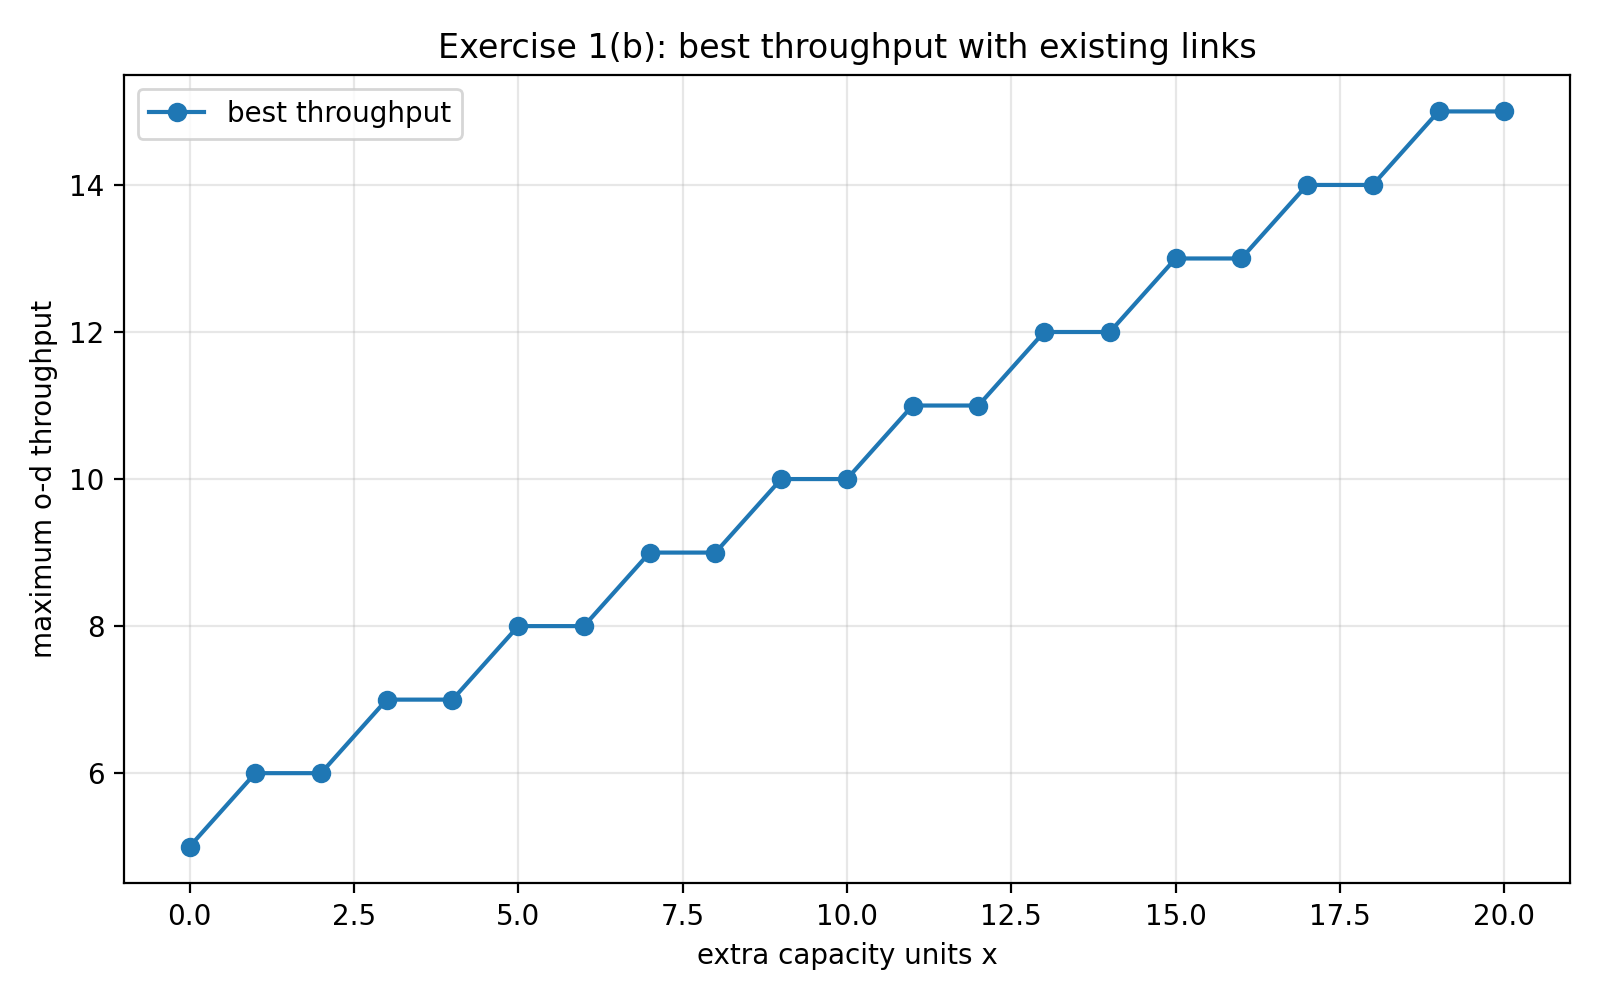
\includegraphics[width=0.75\textwidth]{exercise1_b_throughput.png}
\caption{Best \(o\)-to-\(d\) throughput when the extra capacity is allocated
only on existing links.}
\label{fig:exercise1-b-throughput}
\end{figure}

The throughput increases from \(5\) at \(x=0\) to \(15\) at \(x=20\). The
increase is not one unit for every additional unit of capacity: some capacity
additions must be paired across source-side and sink-side bottlenecks before
they raise the max-flow value.

\subsection*{Adding one new link}

In part 1(c), one new directed link with base capacity \(1\) is first added
between two distinct nodes that are not already connected by an existing
directed edge. Then the same integer extra-capacity budget
\(x=0,\ldots,20\) is allocated over the enlarged edge set. For \(x=0\), the
best added link is \(b\to d\) and the best throughput is \(6\). For
\(x=1,\ldots,20\), the best added link is \(o\to d\), giving throughputs
\[
\begin{array}{c|ccccccccccccccccccccc}
x & 0&1&2&3&4&5&6&7&8&9&10&11&12&13&14&15&16&17&18&19&20\\
\hline
\text{throughput} & 6&7&8&9&10&11&12&13&14&15&16&17&18&19&20&21&22&23&24&25&26
\end{array}
\]
Figure~\ref{fig:exercise1-c-throughput} compares this added-link case with the
existing-link augmentation case.

\begin{figure}[h]
\centering
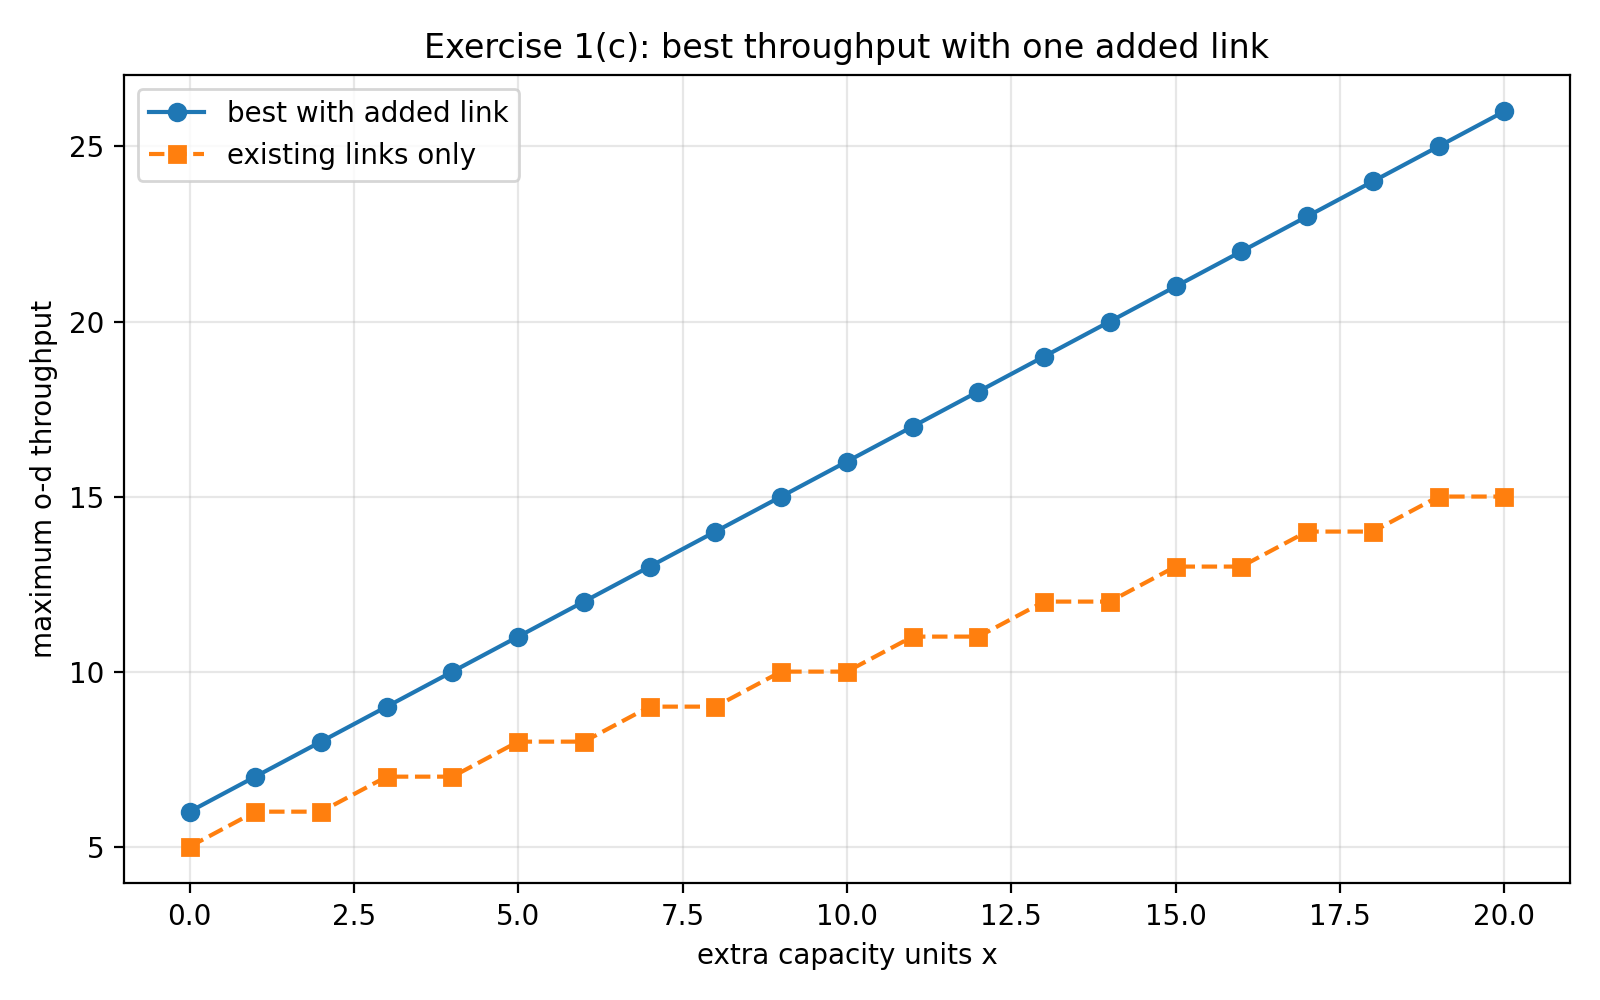
\includegraphics[width=0.75\textwidth]{exercise1_c_added_link_throughput.png}
\caption{Best \(o\)-to-\(d\) throughput when one new directed link is allowed
before allocating the extra capacity.}
\label{fig:exercise1-c-throughput}
\end{figure}

The added-link design is strictly better for every tested budget. The
improvement over the existing-link-only case is \(1\) at \(x=0\), \(1\) at
\(x=1\), and reaches \(11\) at \(x=20\). The result shows that the original
network is limited not only by total installed capacity but also by where that
capacity is located: allowing a direct \(o\to d\) link removes the need to
route new capacity through the original bottleneck structure.

\section{Exercise 2 -- Katz centrality and PageRank}

The graph was reconstructed as a simple undirected graph on
\(\{n_1,\ldots,n_{15}\}\). No visually ambiguous edges were marked in the
reconstruction. The assumed edge set is
\[
\begin{aligned}
E=\{&
n_1n_2,n_1n_3,n_1n_4,n_1n_5,n_1n_6,
n_2n_3,n_2n_4,n_2n_5,n_2n_6,\\
&n_3n_4,n_3n_5,n_3n_6,
n_4n_5,n_4n_6,n_5n_6,
n_6n_{15},n_6n_7,\\
&n_7n_8,n_8n_9,
n_9n_{10},n_9n_{11},n_9n_{12},n_9n_{13},n_9n_{14}\}.
\end{aligned}
\]
Thus the graph has \(15\) nodes and \(24\) undirected edges. In particular,
\(\{n_1,\ldots,n_6\}\) form a clique, node \(n_6\) connects this clique to
\(n_7\) and \(n_{15}\), and node \(n_9\) is the center of a star attached
through the path \(n_6-n_7-n_8-n_9\).

\subsection*{Katz centrality}

Let \(W\) be the adjacency matrix of the reconstructed undirected graph and let
\(\mu\) be the uniform intrinsic centrality vector. Katz centrality was computed
from
\[
x=(I-\beta W)^{-1}\mu .
\]
For \(\beta=0.15\), the largest eigenvalue of \(W\) is
\(\lambda_{\max}(W)=5.0710614673\), so
\[
\frac{1}{\lambda_{\max}(W)}=0.1971973731.
\]
The spectral condition \(\beta<1/\lambda_{\max}(W)\) is therefore satisfied.
The resulting Katz values are shown in Table~\ref{tab:exercise2-katz}; the same
values are plotted in Figure~\ref{fig:exercise2-katz}.

\begin{table}[h]
\centering
\begin{tabular}{c|c|c|c}
\hline
Rank & Node & Degree & Katz\\
\hline
1 & \(n_6\) & 7 & 0.3177933766\\
2 & \(n_1\) & 5 & 0.2858391829\\
2 & \(n_2\) & 5 & 0.2858391829\\
2 & \(n_3\) & 5 & 0.2858391829\\
2 & \(n_4\) & 5 & 0.2858391829\\
2 & \(n_5\) & 5 & 0.2858391829\\
7 & \(n_9\) & 6 & 0.1498337716\\
8 & \(n_7\) & 2 & 0.1306464788\\
9 & \(n_{15}\) & 1 & 0.1143356732\\
10 & \(n_8\) & 2 & 0.1087387042\\
11 & \(n_{10}\) & 1 & 0.0891417324\\
11 & \(n_{11}\) & 1 & 0.0891417324\\
11 & \(n_{12}\) & 1 & 0.0891417324\\
11 & \(n_{13}\) & 1 & 0.0891417324\\
11 & \(n_{14}\) & 1 & 0.0891417324\\
\hline
\end{tabular}
\caption{Katz centrality for \(\beta=0.15\).}
\label{tab:exercise2-katz}
\end{table}

\begin{figure}[h]
\centering
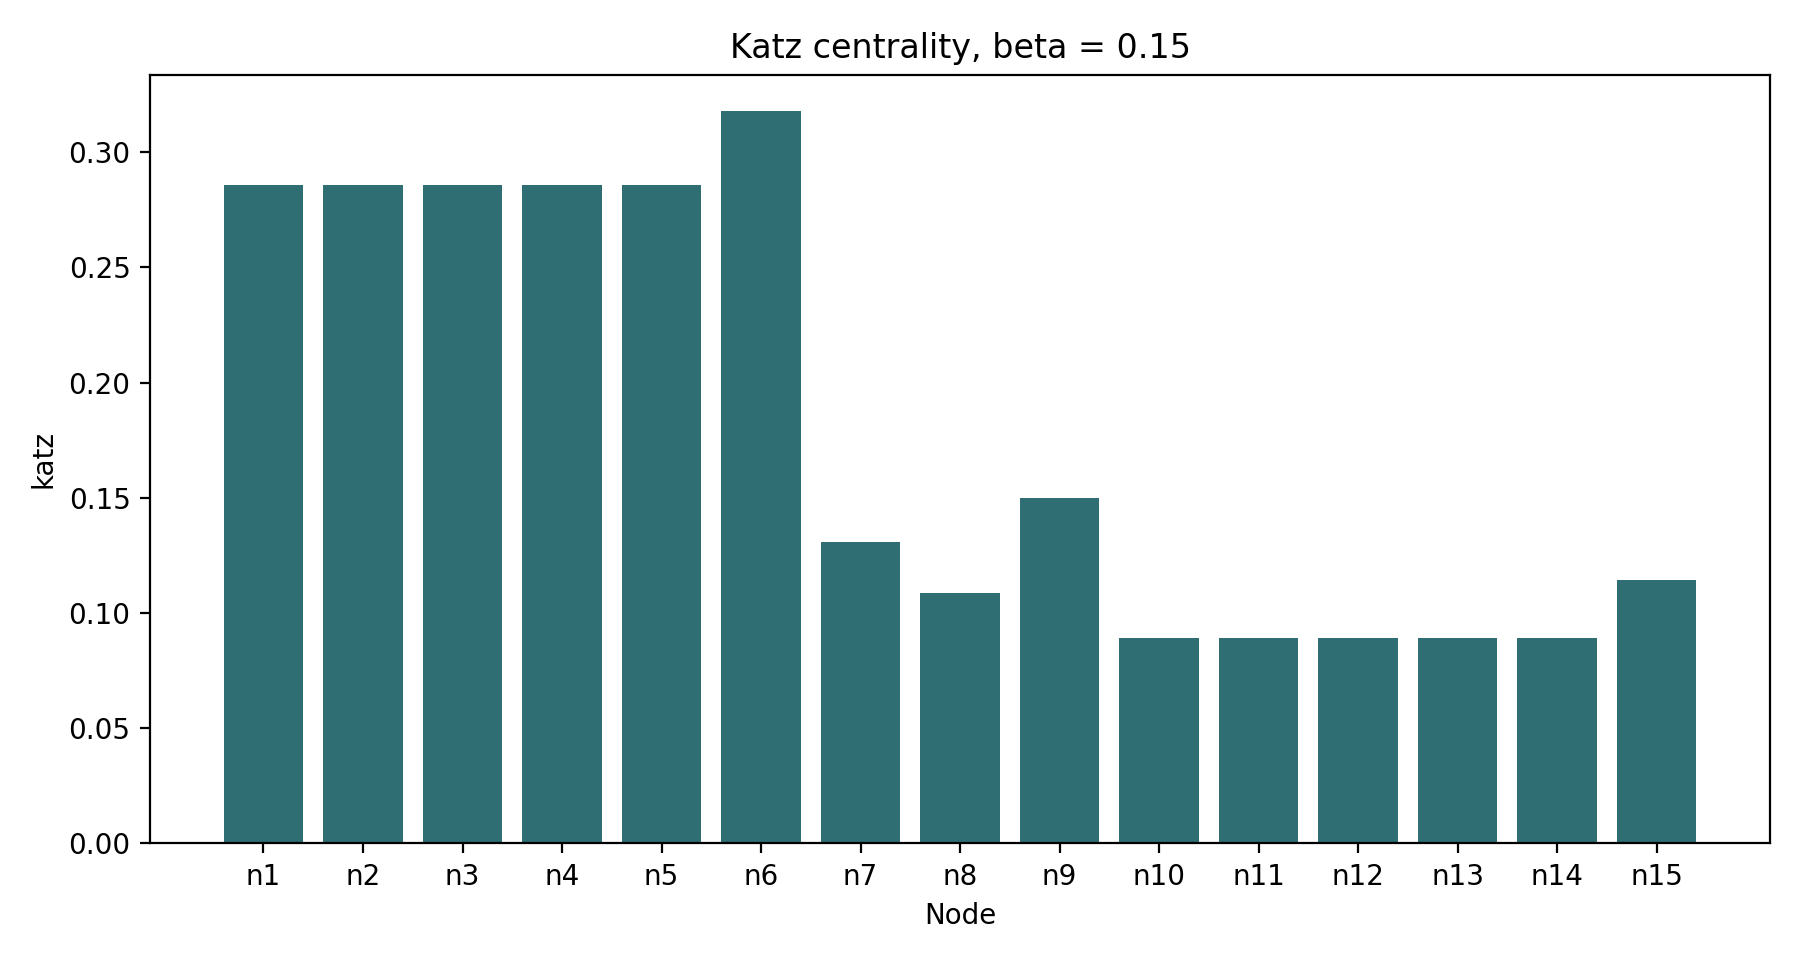
\includegraphics[width=0.75\textwidth]{exercise2_katz.png}
\caption{Katz centrality for the reconstructed graph with \(\beta=0.15\).}
\label{fig:exercise2-katz}
\end{figure}

\subsection*{Distributed PageRank}

For PageRank, each node iterates the distributed update
\[
x_i(t+1)=(1-\beta)\mu_i+\beta\sum_{j\in N(i)}
\frac{x_j(t)}{\deg(j)} .
\]
Equivalently, each node \(j\) sends the normalized quantity
\(x_j(t)/\deg(j)\) to each neighbor. Hence node \(i\) only needs, from each
neighbor \(j\), the current PageRank value \(x_j(t)\) and the neighbor degree
\(\deg(j)\), or directly the already normalized message \(x_j(t)/\deg(j)\).
It then sums these incoming neighbor messages and adds its intrinsic term
\((1-\beta)\mu_i\).

With \(\beta=0.15\), tolerance \(10^{-12}\), and uniform \(\mu\), the method
converged in \(15\) iterations, with final \(L^1\) difference
\(2.011\cdot 10^{-13}\). The PageRank values are reported in
Table~\ref{tab:exercise2-pagerank}; Figure~\ref{fig:exercise2-pagerank} shows
the corresponding plot.

\begin{table}[h]
\centering
\begin{tabular}{c|c|c|c}
\hline
Rank & Node & Degree & PageRank\\
\hline
1 & \(n_9\) & 6 & 0.1059574692\\
2 & \(n_6\) & 7 & 0.0801149613\\
3 & \(n_1\) & 5 & 0.0663447907\\
3 & \(n_2\) & 5 & 0.0663447907\\
3 & \(n_3\) & 5 & 0.0663447907\\
3 & \(n_4\) & 5 & 0.0663447907\\
3 & \(n_5\) & 5 & 0.0663447907\\
8 & \(n_8\) & 2 & 0.0640546671\\
9 & \(n_7\) & 2 & 0.0631875159\\
10 & \(n_{10}\) & 1 & 0.0593156034\\
10 & \(n_{11}\) & 1 & 0.0593156034\\
10 & \(n_{12}\) & 1 & 0.0593156034\\
10 & \(n_{13}\) & 1 & 0.0593156034\\
10 & \(n_{14}\) & 1 & 0.0593156034\\
15 & \(n_{15}\) & 1 & 0.0583834158\\
\hline
\end{tabular}
\caption{Distributed PageRank for \(\beta=0.15\).}
\label{tab:exercise2-pagerank}
\end{table}

\begin{figure}[h]
\centering
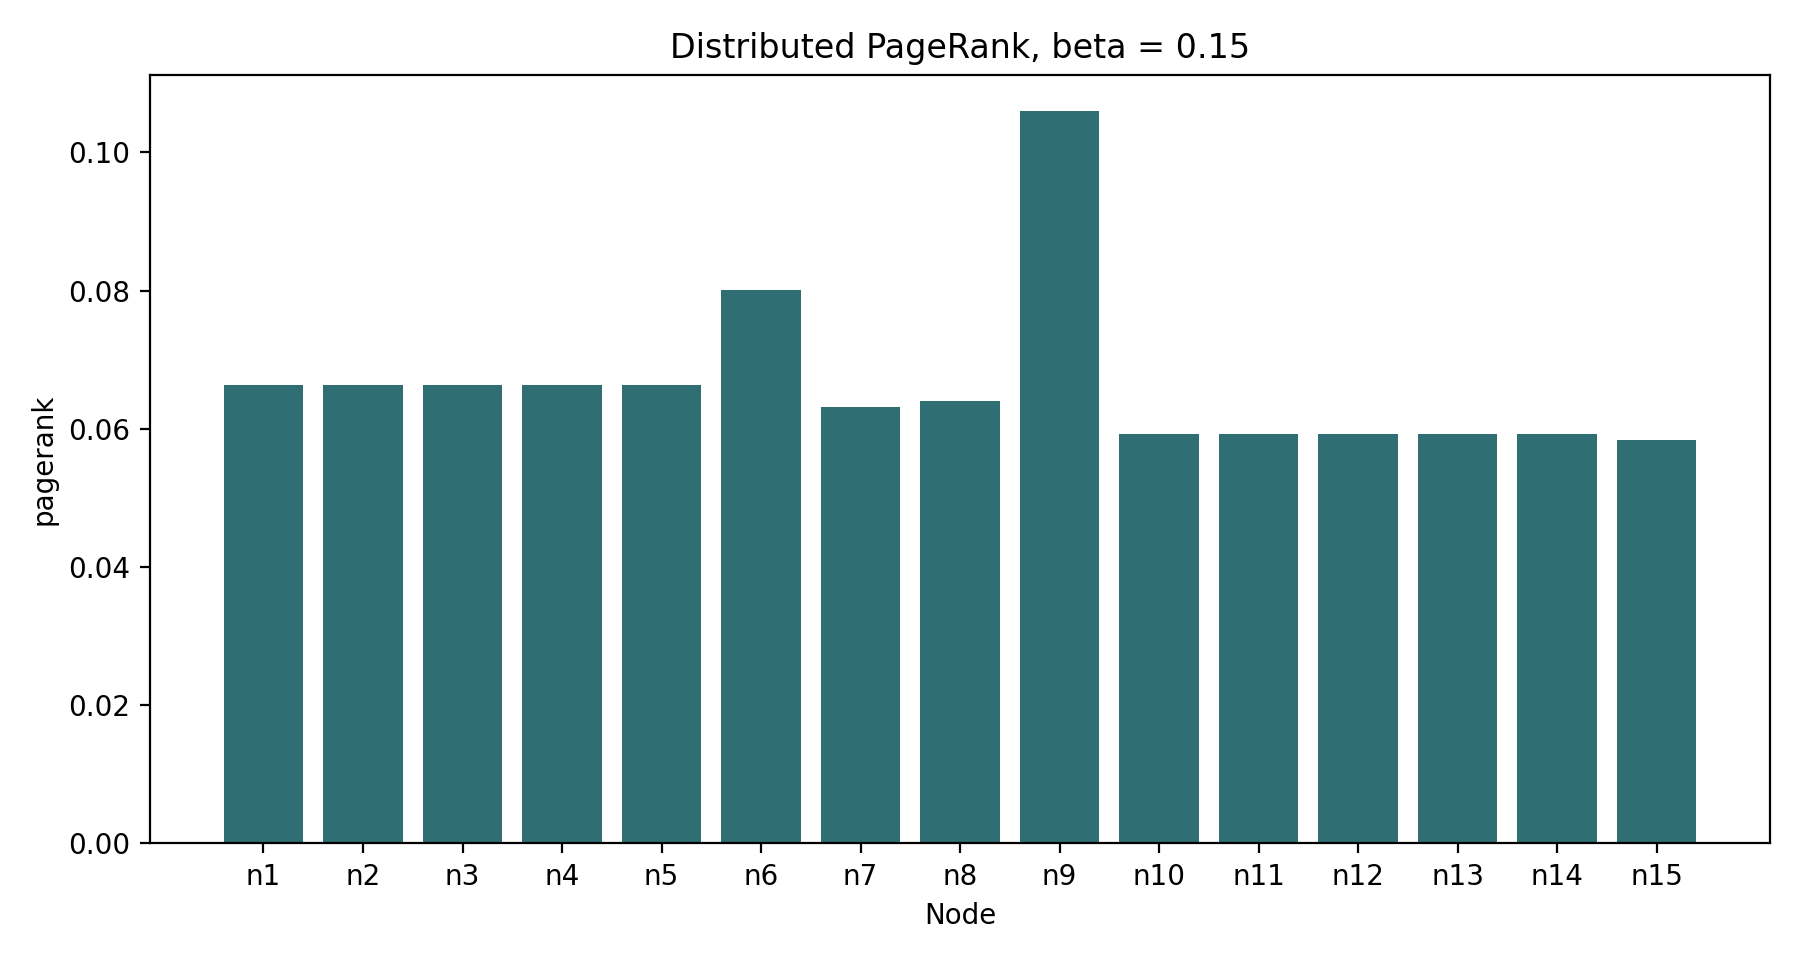
\includegraphics[width=0.75\textwidth]{exercise2_pagerank_beta015.png}
\caption{Distributed PageRank for the reconstructed graph with \(\beta=0.15\).}
\label{fig:exercise2-pagerank}
\end{figure}

\subsection*{Comparison of \(n_6\) and \(n_9\)}

The two nodes have different behavior under Katz centrality and PageRank:
\[
\begin{array}{c|c|c|c|l}
\hline
\text{node} & \text{degree} & \text{Katz} & \text{PageRank} & \text{neighbors}\\
\hline
n_6 & 7 & 0.3177933766 & 0.0801149613
& n_1,n_2,n_3,n_4,n_5,n_7,n_{15}\\
n_9 & 6 & 0.1498337716 & 0.1059574692
& n_8,n_{10},n_{11},n_{12},n_{13},n_{14}\\
\hline
\end{array}
\]
Katz ranks \(n_6\) above \(n_9\). This is because Katz centrality counts raw
walk contributions, and \(n_6\) is embedded in the dense six-node clique while
also acting as the bridge toward the path and \(n_{15}\). PageRank ranks
\(n_9\) above \(n_6\). The reason is the degree normalization in the PageRank
update: the degree-one leaves \(n_{10},\ldots,n_{14}\) send all their PageRank
mass to \(n_9\), whereas the clique nodes adjacent to \(n_6\) split their mass
among five neighbors.

\subsection*{PageRank sensitivity to \(\beta\)}

The PageRank comparison between \(n_6\) and \(n_9\) was repeated for
\(\beta\in\{0,1/4,1/2,3/4,1\}\). The results are shown in
Table~\ref{tab:exercise2-beta}. At \(\beta=0\), only the uniform intrinsic
centrality matters, so all nodes have PageRank \(1/15=0.0666666667\). At
\(\beta=1\), the score is determined only by the graph random-walk structure.

\begin{table}[h]
\centering
\begin{tabular}{c|c|c|c|c}
\hline
\(\beta\) & \(PR(n_6)\) & \(PR(n_9)\) & \(PR(n_6)-PR(n_9)\) & Iterations\\
\hline
0.00 & 0.0666666667 & 0.0666666667 & 0.0000000000 & 1\\
0.25 & 0.0875066385 & 0.1269777272 & -0.0394710887 & 20\\
0.50 & 0.1014039855 & 0.1666925466 & -0.0652885611 & 38\\
0.75 & 0.1106044872 & 0.1911159378 & -0.0805114506 & 88\\
1.00 & 0.1458333333 & 0.1250000000 & 0.0208333333 & 1083\\
\hline
\end{tabular}
\caption{PageRank sensitivity for nodes \(n_6\) and \(n_9\).}
\label{tab:exercise2-beta}
\end{table}

\begin{figure}[h]
\centering
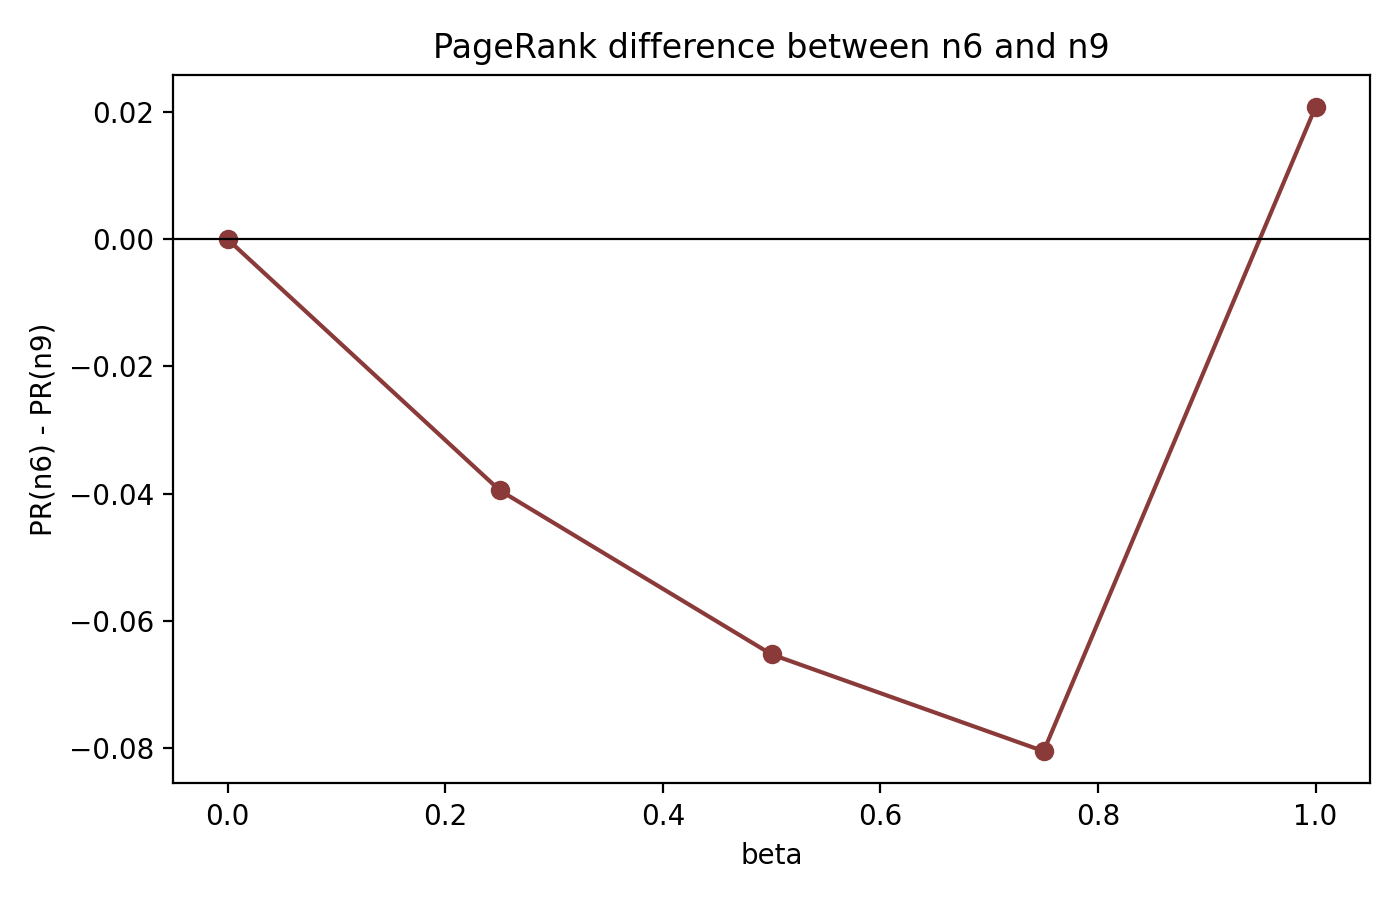
\includegraphics[width=0.75\textwidth]{exercise2_pagerank_difference_beta.png}
\caption{Difference \(PR(n_6)-PR(n_9)\) as a function of \(\beta\).}
\label{fig:exercise2-beta-difference}
\end{figure}

The tested sequence \(PR(n_6)-PR(n_9)\) is not monotone in \(\beta\): it first
decreases from \(0\) to \(-0.0805114506\), then increases to
\(0.0208333333\) at \(\beta=1\).

\section{Exercise 3 -- Traffic assignment}

The traffic network is a directed graph with \(17\) nodes and \(28\) directed
links. The data are loaded from the four matrix files: the measured flow
vector \(f\), the capacity vector \(C\), the incidence matrix \(B\), and the
free-flow travel-time vector \(l\). The incidence matrix has one column per
link and one row per node. In each link column, \(+1\) marks the tail node and
\(-1\) marks the head node. Reconstructing the directed links from \(B\)
therefore gives exactly the \(28\) links used in the graph computations.

For link \(e\), the travel-time function is
\[
\tau_e(f_e)=\frac{l_e}{1-f_e/C_e}, \qquad 0\leq f_e<C_e.
\]
In the convex programs below, the numerical constraint
\[
0\leq f_e\leq 0.999 C_e
\]
is imposed on every link.

\subsection*{Shortest path and maximum flow}

Using the free-flow times \(l_e\) as edge weights, the shortest path from node
\(1\) to node \(17\) is
\[
1\to 2\to 3\to 9\to 13\to 17,
\]
using links
\[
1,\ 2,\ 12,\ 9,\ 25.
\]
The total free-flow travel time on this path is \(0.559833\).

Using the capacities \(C_e\), the maximum \(1\)-to-\(17\) flow is
\[
22448.000000.
\]

\subsection*{Exogenous inflow vector}

The original node imbalance is computed from the measured flow by
\[
\nu = Bf.
\]
For the optimization problems, only the net source inflow at node \(1\) and
the corresponding sink outflow at node \(17\) are kept:
\[
\nu^{\mathrm{new}}_1=\nu_1=16806,\qquad
\nu^{\mathrm{new}}_{17}=-16806,
\]
and all other entries are set to zero. Table~\ref{tab:exercise3-nu} reports
both vectors.

\begin{table}[h]
\centering
\begin{tabular}{c|r|r}
\hline
Node & \(\nu=Bf\) & \(\nu^{\mathrm{new}}\)\\
\hline
1 & 16806 & 16806\\
2 & 8570 & 0\\
3 & 19448 & 0\\
4 & 4957 & 0\\
5 & -746 & 0\\
6 & 4768 & 0\\
7 & 413 & 0\\
8 & -2 & 0\\
9 & -5671 & 0\\
10 & 1169 & 0\\
11 & -5 & 0\\
12 & -7131 & 0\\
13 & -380 & 0\\
14 & -7412 & 0\\
15 & -7810 & 0\\
16 & -3430 & 0\\
17 & -23544 & -16806\\
\hline
\end{tabular}
\caption{Original and reduced exogenous inflow vectors.}
\label{tab:exercise3-nu}
\end{table}

\subsection*{Social optimum}

The social optimum minimizes total travel time:
\[
\begin{aligned}
\min_f \quad & \sum_e f_e \tau_e(f_e)\\
\text{s.t.}\quad & Bf=\nu^{\mathrm{new}},\\
&0\leq f\leq 0.999C .
\end{aligned}
\]
For the given delay function, the equivalent convex objective used in CVXPY is
\[
\sum_e \left(\frac{l_e C_e}{1-f_e/C_e}-l_e C_e\right).
\]
The solver status was \(\mathrm{optimal}\). The optimal total travel time was
\[
26142.669150.
\]

\subsection*{Wardrop equilibrium}

The Wardrop equilibrium is obtained by minimizing the Beckmann potential
\[
\begin{aligned}
\min_f \quad & \sum_e -l_e C_e\log(1-f_e/C_e)\\
\text{s.t.}\quad & Bf=\nu^{\mathrm{new}},\\
&0\leq f\leq 0.999C .
\end{aligned}
\]
The solver status was again \(\mathrm{optimal}\). The total travel time at the
Wardrop equilibrium was
\[
26495.321759.
\]
Compared with the social optimum, this gives the price of anarchy
\[
\frac{26495.321759}{26142.669150}=1.013490.
\]
Thus the selfish-routing equilibrium has about \(1.349\%\) larger total travel
time than the social optimum.

\subsection*{Marginal-cost tolls}

To decentralize the social optimum, marginal-cost tolls are set to
\[
\omega_e=f^{\star}_e \tau'_e(f^{\star}_e),
\qquad
\tau'_e(f_e)=\frac{l_e/C_e}{(1-f_e/C_e)^2}.
\]
The tolled Wardrop problem minimizes
\[
\sum_e -l_e C_e\log(1-f_e/C_e)+\sum_e \omega_e f_e
\]
under the same flow-conservation and capacity constraints. The tolled Wardrop
solver status was \(\mathrm{optimal}\), and the verification error was
\[
\|f^{\mathrm{tolled}}-f^\star\|_2=2.993561\cdot 10^{-1}.
\]
Since the flows are on the order of thousands of vehicles, this norm is a
small numerical discrepancy, confirming that the marginal-cost tolls recover
the social optimum up to solver tolerance.

\subsection*{Additional-delay objective and tolls}

The additional-delay objective subtracts free-flow time from each link cost:
\[
\psi_e(f_e)=f_e(\tau_e(f_e)-l_e).
\]
The optimization problem is
\[
\begin{aligned}
\min_f \quad & \sum_e \psi_e(f_e)\\
\text{s.t.}\quad & Bf=\nu^{\mathrm{new}},\\
&0\leq f\leq 0.999C .
\end{aligned}
\]
The optimum solver status was \(\mathrm{optimal}\), with objective value
\[
15350.353857.
\]
The tolls that decentralize this optimum are
\[
\omega^{\mathrm{add}}_e
=\psi'_e(f^{\star,\mathrm{add}}_e)-\tau_e(f^{\star,\mathrm{add}}_e)
=-l_e+f^{\star,\mathrm{add}}_e\tau'_e(f^{\star,\mathrm{add}}_e).
\]
The corresponding tolled Wardrop solver status was \(\mathrm{optimal}\), and
\[
\|f^{\mathrm{tolled,add}}-f^{\star,\mathrm{add}}\|_2
=5.658613\cdot 10^{-1}.
\]
This is again small relative to the link flows, so the additional-delay tolls
recover the additional-delay optimum within numerical accuracy.

\begin{table}[h]
\centering
\begin{tabular}{l|r}
\hline
Quantity & Value\\
\hline
Social optimum total travel time & 26142.669150\\
Wardrop total travel time & 26495.321759\\
Price of anarchy & 1.013490\\
Additional-delay optimum objective & 15350.353857\\
\(\|f^{\mathrm{tolled}}-f^\star\|_2\) & \(2.993561\cdot 10^{-1}\)\\
\(\|f^{\mathrm{tolled,add}}-f^{\star,\mathrm{add}}\|_2\) &
\(5.658613\cdot 10^{-1}\)\\
\hline
\end{tabular}
\caption{Main optimization and verification results for Exercise 3.}
\label{tab:exercise3-summary}
\end{table}

\begin{table}[h]
\centering
\scriptsize
\begin{tabular}{c|r|r}
\hline
Edge & \(\omega\) & \(\omega^{\mathrm{add}}\)\\
\hline
1 & 1.973436 & 1.843996\\
2 & 0.193184 & 0.110524\\
3 & 0.049432 & -0.070804\\
4 & 0.100106 & -0.066454\\
5 & 1.512756 & 1.367481\\
6 & 0.483666 & 0.406893\\
7 & 0.112309 & 0.027030\\
8 & 0.059648 & 0.008671\\
9 & 0.271745 & 0.101759\\
10 & 0.008287 & -0.093639\\
11 & 0.000000 & -0.106670\\
12 & 0.067438 & -0.059339\\
13 & 0.000000 & -0.112330\\
14 & 0.120075 & -0.034066\\
15 & 0.498195 & 0.369956\\
16 & 0.084654 & 0.017702\\
17 & 0.073394 & -0.003661\\
18 & 0.019181 & -0.035492\\
19 & 0.001514 & -0.031226\\
20 & 0.013113 & -0.024622\\
21 & 0.067738 & 0.009238\\
22 & 0.257081 & 0.123439\\
23 & 0.066941 & -0.020805\\
24 & 0.000000 & -0.054167\\
25 & 0.391850 & 0.272065\\
26 & 0.269515 & 0.228422\\
27 & 0.147694 & 0.025865\\
28 & 0.597989 & 0.423527\\
\hline
\end{tabular}
\caption{Marginal-cost tolls for the social optimum and tolls for the
additional-delay optimum.}
\label{tab:exercise3-tolls}
\end{table}

\begin{table}[h]
\centering
\scriptsize
\begin{tabular}{c|c|r|r|r|r|r}
\hline
Edge & Arc & \(f^\star\) & \(f^{W}\) & \(f^{\mathrm{tolled}}\) &
\(f^{\star,\mathrm{add}}\) & \(f^{\mathrm{tolled,add}}\)\\
\hline
1 & \(1\to2\) & 6569.213 & 6557.510 & 6569.053 & 6584.465 & 6584.310\\
2 & \(2\to3\) & 5809.999 & 6308.594 & 5809.976 & 5577.902 & 5578.047\\
3 & \(3\to4\) & 3046.970 & 2200.641 & 3046.966 & 3367.453 & 3367.367\\
4 & \(4\to5\) & 3046.970 & 2200.641 & 3046.966 & 3367.453 & 3367.367\\
5 & \(1\to6\) & 10236.787 & 10248.490 & 10236.947 & 10221.535 & 10221.690\\
6 & \(6\to7\) & 4666.496 & 4706.686 & 4666.565 & 4669.458 & 4669.522\\
7 & \(7\to8\) & 3061.217 & 2859.927 & 3061.219 & 3156.434 & 3156.371\\
8 & \(8\to9\) & 2595.955 & 2232.651 & 2595.958 & 2711.828 & 2711.726\\
9 & \(9\to13\) & 3104.550 & 3350.007 & 3104.548 & 2987.937 & 2987.976\\
10 & \(2\to7\) & 759.214 & 248.916 & 759.077 & 1006.563 & 1006.263\\
11 & \(3\to8\) & 0.000 & 11.665 & 0.000 & 0.000 & 0.000\\
12 & \(3\to9\) & 2763.029 & 4096.288 & 2763.010 & 2210.449 & 2210.680\\
13 & \(4\to9\) & 0.000 & 0.000 & 0.000 & 0.000 & 0.000\\
14 & \(5\to14\) & 3046.970 & 2200.641 & 3046.966 & 3367.453 & 3367.367\\
15 & \(6\to10\) & 5570.291 & 5541.804 & 5570.382 & 5552.076 & 5552.168\\
16 & \(10\to11\) & 2893.839 & 2343.349 & 2893.856 & 3084.751 & 3084.683\\
17 & \(10\to15\) & 5040.945 & 5294.130 & 5040.949 & 4986.912 & 4986.898\\
18 & \(7\to10\) & 2364.493 & 2095.675 & 2364.423 & 2519.587 & 2519.413\\
19 & \(8\to11\) & 465.262 & 638.941 & 465.260 & 444.607 & 444.645\\
20 & \(9\to12\) & 2254.434 & 2978.932 & 2254.420 & 1934.340 & 1934.430\\
21 & \(11\to12\) & 3359.102 & 2982.290 & 3359.116 & 3529.358 & 3529.328\\
22 & \(12\to13\) & 5613.535 & 5961.222 & 5613.536 & 5463.697 & 5463.758\\
23 & \(13\to14\) & 2371.991 & 2522.440 & 2371.992 & 2202.316 & 2202.404\\
24 & \(11\to15\) & 0.000 & 0.000 & 0.000 & 0.000 & 0.000\\
25 & \(13\to17\) & 6346.094 & 6788.789 & 6346.093 & 6249.318 & 6249.331\\
26 & \(14\to17\) & 5418.960 & 4723.081 & 5418.958 & 5569.769 & 5569.771\\
27 & \(15\to16\) & 5040.945 & 5294.130 & 5040.949 & 4986.912 & 4986.898\\
28 & \(16\to17\) & 5040.945 & 5294.130 & 5040.949 & 4986.912 & 4986.898\\
\hline
\end{tabular}
\caption{Edge-flow comparison for the social optimum, Wardrop equilibrium,
marginal-cost tolled Wardrop, additional-delay optimum, and additional-delay
tolled Wardrop.}
\label{tab:exercise3-flows}
\end{table}

\begin{figure}[h]
\centering
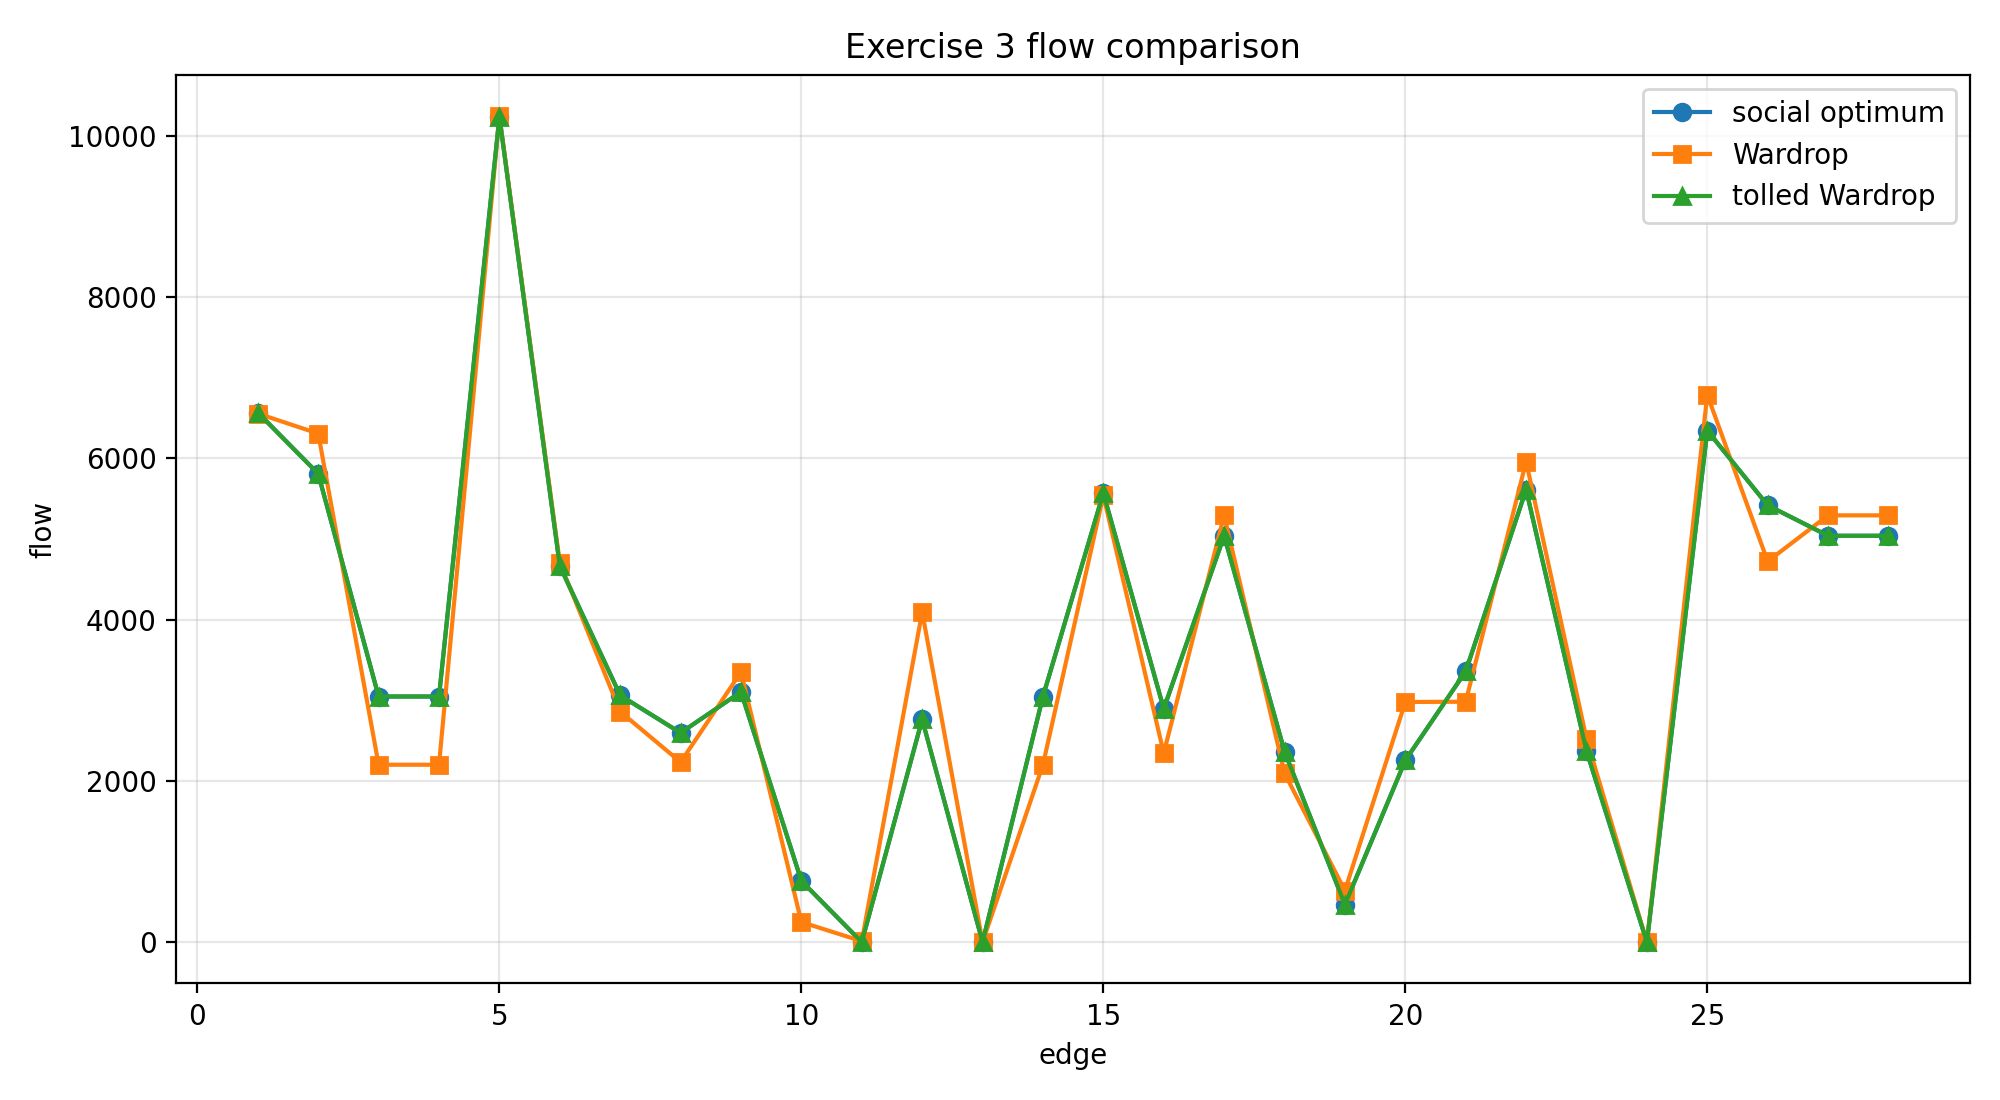
\includegraphics[width=0.8\textwidth]{exercise3_flow_comparison.png}
\caption{Flow comparison between the social optimum, untolled Wardrop
equilibrium, and marginal-cost tolled Wardrop equilibrium.}
\label{fig:exercise3-flow-comparison}
\end{figure}

\section{Conclusion}

Exercise 1 confirmed the max-flow/min-cut theorem on the small directed
network: the minimum cut capacity and maximum flow are both \(5\). Integer
capacity augmentation on existing links increases throughput from \(5\) to
\(15\) over the tested budgets, while allowing one new directed link gives a
larger throughput for every tested budget and reaches \(26\) at \(x=20\).

Exercise 2 showed that Katz centrality and PageRank emphasize different
structural roles. Katz centrality ranks \(n_6\) highest because it is embedded
in the dense clique and also connects to the rest of the graph. PageRank ranks
\(n_9\) highest for \(\beta=0.15\), because several degree-one neighbors send
all their normalized mass to \(n_9\). The sensitivity test showed that
\(PR(n_6)-PR(n_9)\) is not monotone in \(\beta\).

Exercise 3 compared routing objectives on the traffic network. The Wardrop
equilibrium has total travel time \(26495.321759\), compared with
\(26142.669150\) at the social optimum, giving a price of anarchy of
\(1.013490\). The marginal-cost tolls and the additional-delay tolls both
recover their target optima within small numerical discrepancies relative to
the scale of the link flows.

\appendix
\section{Reproducibility appendix}

All commands are intended to be run from the project root directory
\texttt{hw1/}. The data files used by Exercise 3 are stored in
\texttt{data/}: \texttt{flow.mat}, \texttt{capacities.mat},
\texttt{traffic.mat}, and \texttt{traveltime.mat}.

The Python dependencies are \texttt{numpy}, \texttt{scipy},
\texttt{networkx}, \texttt{cvxpy}, \texttt{matplotlib}, and
\texttt{pandas}. A typical installation command is
\begin{quote}
\texttt{pip install numpy scipy networkx cvxpy matplotlib pandas}
\end{quote}

The scripts are executed as
\begin{quote}
\texttt{python src/exercise1.py}\\
\texttt{python src/exercise2.py}\\
\texttt{python src/exercise3.py}
\end{quote}
They regenerate the CSV files in \texttt{results/} and the plots in
\texttt{figures/}. The final report can be compiled from the project root with
\begin{quote}
\texttt{pdflatex -interaction=nonstopmode -output-directory=report report/report.tex}
\end{quote}

The main result files are:
\begin{itemize}
\item Exercise 1: \texttt{exercise1\_cuts.csv},
\texttt{exercise1\_b\_results.csv}, and
\texttt{exercise1\_c\_results.csv}.
\item Exercise 2: \texttt{exercise2\_katz.csv},
\texttt{exercise2\_pagerank\_beta015.csv}, and
\texttt{exercise2\_pagerank\_beta\_sensitivity.csv}.
\item Exercise 3: \texttt{exercise3\_shortest\_path.csv},
\texttt{exercise3\_maxflow.csv}, \texttt{exercise3\_nu.csv},
\texttt{exercise3\_social\_optimum.csv}, \texttt{exercise3\_wardrop.csv},
\texttt{exercise3\_tolls\_total\_travel\_time.csv}, and
\texttt{exercise3\_additional\_delay.csv}.
\end{itemize}

The figures referenced in the report are:
\begin{itemize}
\item \texttt{figures/exercise1\_b\_throughput.png}
\item \texttt{figures/exercise1\_c\_added\_link\_throughput.png}
\item \texttt{figures/exercise2\_katz.png}
\item \texttt{figures/exercise2\_pagerank\_beta015.png}
\item \texttt{figures/exercise2\_pagerank\_difference\_beta.png}
\item \texttt{figures/exercise3\_flow\_comparison.png}
\end{itemize}

\end{document}
